\subsection{Objektstrukturplan}

Der Objektstrukturplan ist visuell sehr änhlich zum Projektstrukturplan, jedoch werden hier nicht Arbeitspakete dargestellt, sondern die einzelnen Teilkomponenten des Produktes. Der Objektstrukturplan gibt einen Überblick über die einzelnen teilkomponenten Komponenten des Produktes. In \ref{fig:objektstrukturplan_prototyp} wird der Objektstrukturplan des Prototypen dargestellt. \cite{objektstrukturplan}

\begin{figure}[ht]
  \centering
  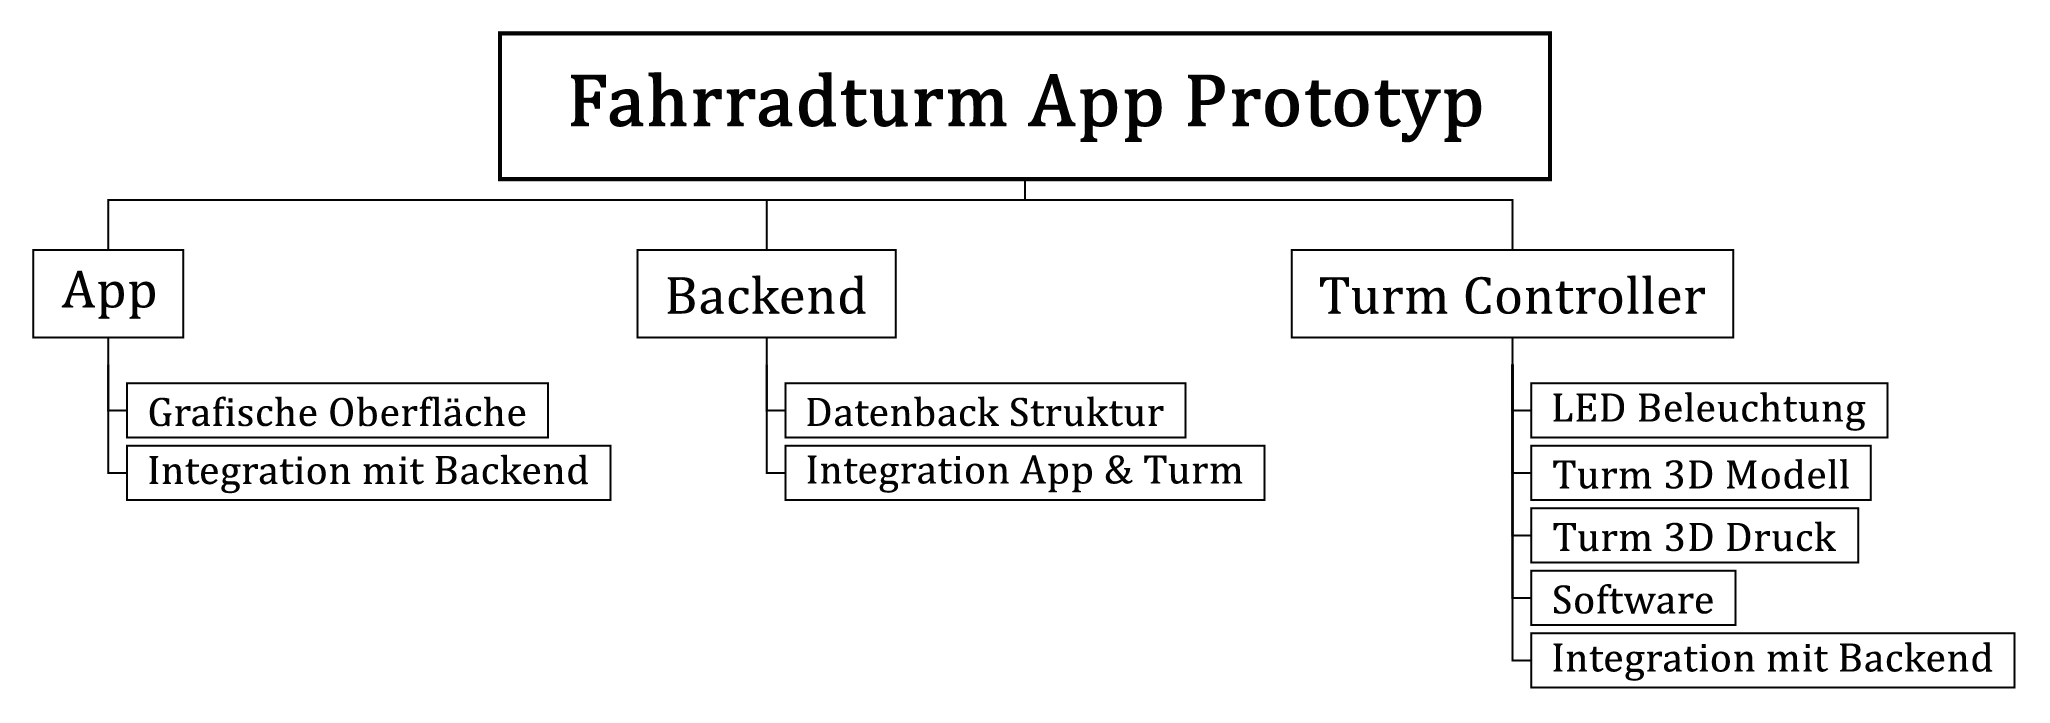
\includegraphics[width=1\textwidth]{images/objektstrukturplan_prototyp}
  \caption{Objektstrukturplan des Prototypen}
  \label{fig:objektstrukturplan_prototyp}
\end{figure}